\section{vigenere密码破译程序}
    以下将介绍在已知vigenere密码的密文的情况下破解其明文以及密钥

\subsection{编写思路}
    \subsubsection{通过重合指数法破解密钥的长度}
        在将密文中的空格去除之后通过find\_key\_len函数遍历从2到50的所有的密钥长度,假设当前遍历的密钥长度为i,
        则将密文分成i组,对于每一组调用count\_key\_len\_CI函数求其重合指数,得到密钥长度为i时的重合指数,因为每一个
        密钥长度对应有数组重合指数,所以在该次实验中调用Bias函数将当前密钥长度的重合指数求其对于0.065的偏差,
        取偏差最小的一组的密钥长度为该密文的密钥长度。\\   

    \subsubsection{通过互重合指数确定密钥字符之间的相对位移}
        在得到了密钥的长度key\_len之后通过调用group\_k函数将密钥字符串分成key\_len组,通过count\_MIC函数
        求得每一组与第一组之间的互重合指数表,并选取表中互重合指数最接近0.065的值的下标作为当前字符相对于第一个
        字符的偏移量,从而得到所有字符相对于第一个字符的偏移量。\\

    \subsubsection{遍历26种密钥字的情况选出合适的密钥字}
        该过程遍历26种密钥的情况,将密文的前二十位字符拿出用26种密钥分别进行解密,将解密的结果进行分词处理,由
        程序员选出最为符合语义的一个密钥并将其输入程序。\\

    \subsubsection{将密文字符串通过密钥转换为明文并做英文的分词处理}
        该步骤是在已知密文已知密钥的情况下将密文字符串进行翻译从而得到明文字符串,然后将得到的明文字符串进行
        分词处理,从而得到一个通顺的句子。\\
\newpage

\subsection{源代码}
    \lstinputlisting[language=Python, caption=vigenere破解程序代码]{codes/vigenere2.py}

\newpage
\subsection{代码运行结果演示}
    \subsubsection{破译过程1}
        已知密文为:\\

        \begin{lstlisting}
        cbkznkiyjsrofgnqadnzuqigscvxizgsjwucusrdkxuahgzrhywtvdjeiuwsrrtnpszbvpzncngztbvsrnzuqigscvf
        jwqgjwcytwdazuqigscvfjwqgjwjhkfdylmcbmhonbmbvdnvbmwbnacjaphhonbmbvdnvbmwbnaublsbdnjjneoroyf
        mxfhixpzpcozzuqigscvxcvhdmfgxmgovzsqmvzyvwyzmsczoajsejifoakdcrehwhgdehvmtnmvvmesvzifutzfjzo
        alwqztunwvdvmfhesvzifutzfjzoalwqztunpsnoyfleoxdetbwfsoyfjmfhjuxuagnarsfqydoyfjzsrzeujmfhjuu
        bihrjdfinwsnepcawdnkbobvnmzucmghijjmbscjejnapddehlmqddmfxncqbfpxwfejifpqzhikiyaiozimubwuzuf
        azsdjwdiudzmztivcmgp
        \end{lstlisting}

        破译结果如下图所示\\
        求得密钥长度和偏移量后遍历26种可能的密钥结果
        \begin{figure}[htbp]
            \centering 
            \begin{subfigure}[b]{0.4\textwidth}
                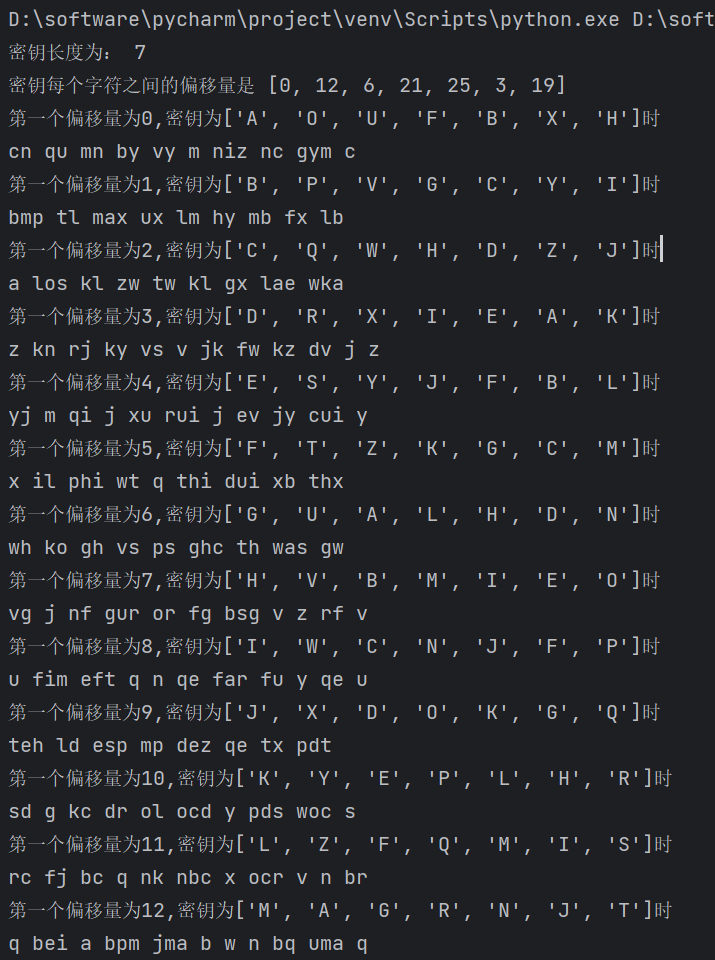
\includegraphics[width=\textwidth]{images/vigenere2_result_1.1.png}
                \label{fig:subfig1}
            \end{subfigure}
            \hfill
            \begin{subfigure}[b]{0.5\textwidth}
                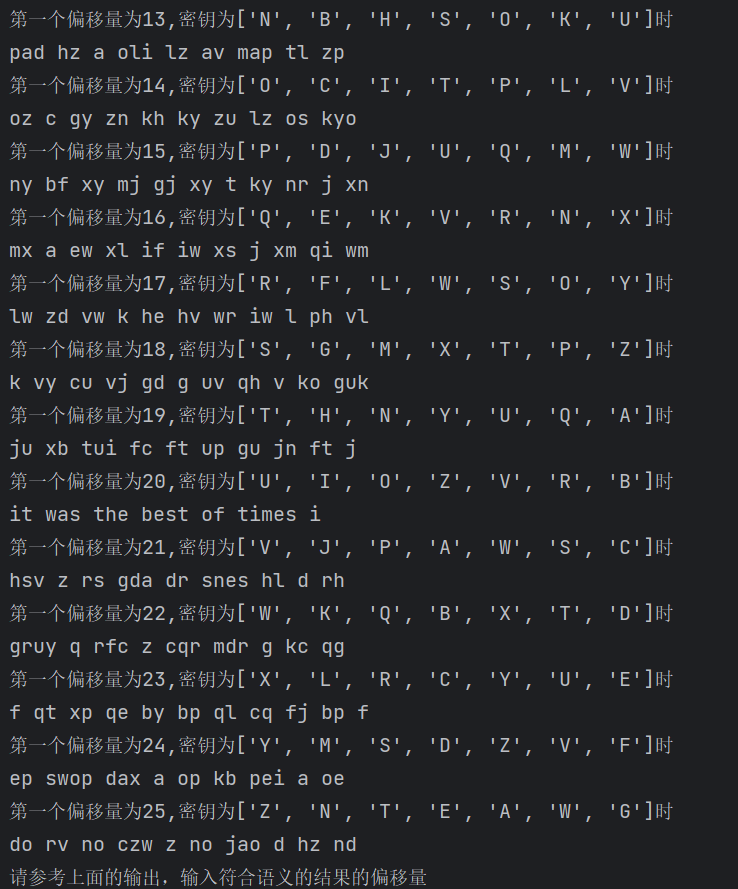
\includegraphics[width=\textwidth]{images/vigenere2_result_1.2.png}
                \label{fig:subfig2}
            \end{subfigure}
        
            \caption{密钥长度,偏移量和26种密钥运行结果}
            \label{fig:subfigures}
        \end{figure}

        选择最为符合语义的密钥结果后输出相应的明文如下图所示
        \begin{figure}[htbp] %代表图片的插入位置h:当前位置,t页面顶部,b页面底部,p浮动页
            \centering    %图片居中
            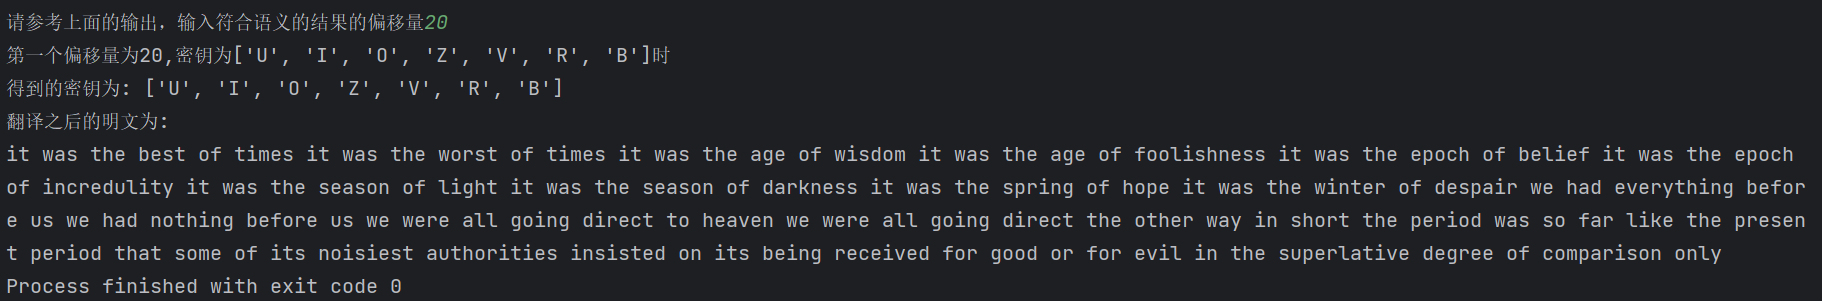
\includegraphics[width=18cm]{images/vigenere2_result1.3.png}  %[可选参数设置图片的宽高]
            \caption{得到明文结果}    %图片标题
            \label{pic1}        %图片标签
        \end{figure}
    \newpage
    \subsubsection{破译过程2}
        已知密文为:\\
        \begin{lstlisting}
            krkpekmcwxtvknugcmkxfwmgmjvpttuflihcumgxafsdajfupgzzmjlkyykxdvccyqiwdncebwhyjmgkazybtdf
            sitncwdnolqiacmchnhwcgxfzlwtxzlvgqecllhimbnudynagrttgiiycmvyyimjzqaxvkcgkgrawxupmjwqemi
            ptzrtmqdciakjudnnuadfrimbbuvyaeqwshtpuyqhxvyaeffldmtvrjkpllsxtrlnvkiajfukycvgjgibubldpp
            kfpmkkuplafslaqycaigushmqxcityrwukqdftkgrlstncudnnuzteqjrxyafshaqljsljfunhwiqtehncpkgxs
            pkfvbstarlsgkxfibffldmerptrqlygxpfrwxtvbdgqkztmtfsqegumcfararhwerchvygczyzjaacgntgvfktm
            jvlpmkflpecjqtfdcclbncqwhycccbgeanyciclxncrwxofqieqmcshhdccughsxxvzdnhwtycmcbcrttvmurql
            phxnwddkopqtehzapgpfrlkkkcpgadmgxdlrchvygczkerwxyfpawefsawukmefgkmpwqicnhwlnihvycsxckf
        \end{lstlisting}

        破译结果如下图所示
        求得密钥长度和偏移量后遍历26种可能的密钥结果
        \begin{figure}[htbp]
            \centering 
            \begin{subfigure}[b]{0.4\textwidth}
                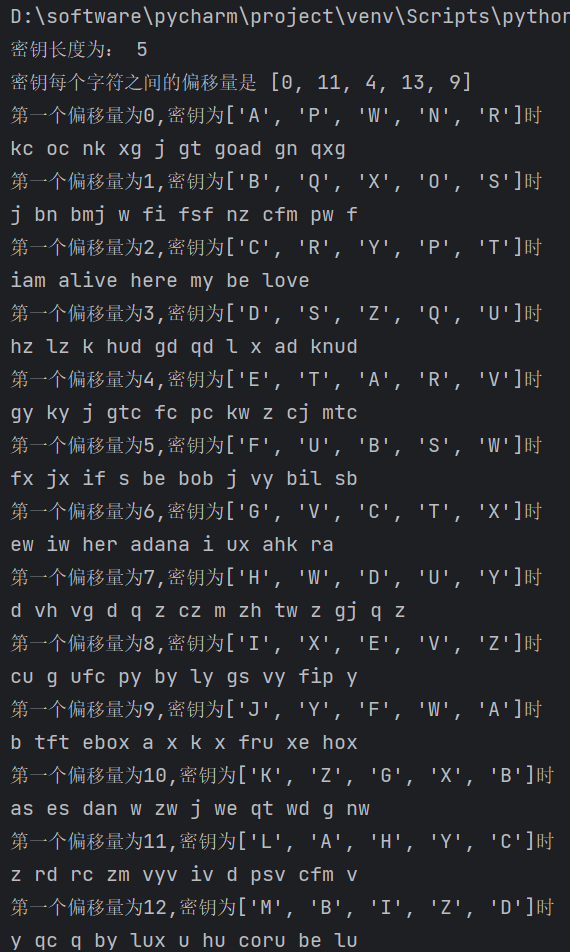
\includegraphics[width=\textwidth]{images/vigenere2_result2_1.1.png}
                \label{fig:subfig1}
            \end{subfigure}
            \hfill
            \begin{subfigure}[b]{0.4\textwidth}
                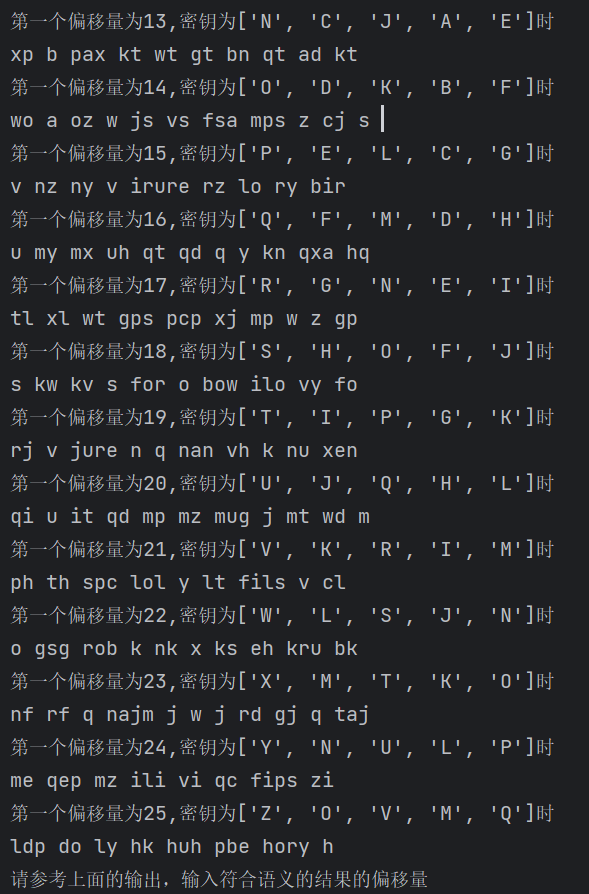
\includegraphics[width=\textwidth]{images/vigenere2_result2_1.2.png}
                \label{fig:subfig2}
            \end{subfigure}
        
            \caption{密钥长度,偏移量和26种密钥运行结果}
            \label{fig:subfigures}
        \end{figure}

        选择最为符合语义的密钥结果后输出相应的明文如下图所示
        \begin{figure}[htbp] %代表图片的插入位置h:当前位置,t页面顶部,b页面底部,p浮动页
            \centering    %图片居中
            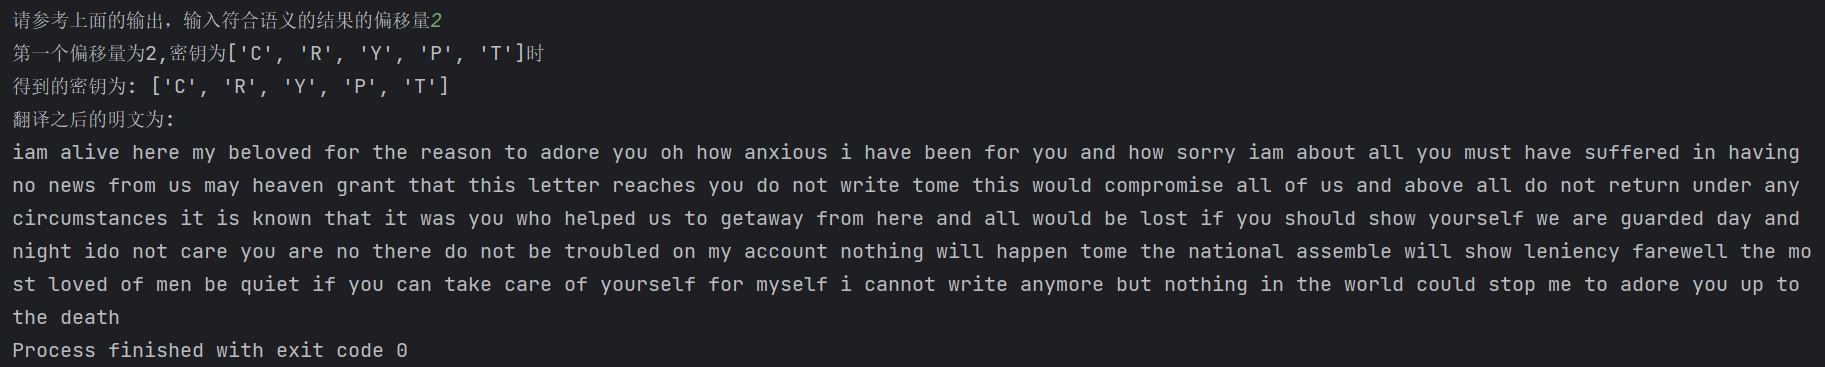
\includegraphics[width=18cm]{images/vigenere2_result2_1.3.png}  %[可选参数设置图片的宽高]
            \caption{得到明文结果}    %图片标题
            \label{pic1}        %图片标签
        \end{figure}